
\begin{frame}[fragile]
\frametitle{Challenge: Cross-References}
\begin{center}
    \textbf{Recreate the following document: }\\
\end{center}
\vspace{0.2cm}
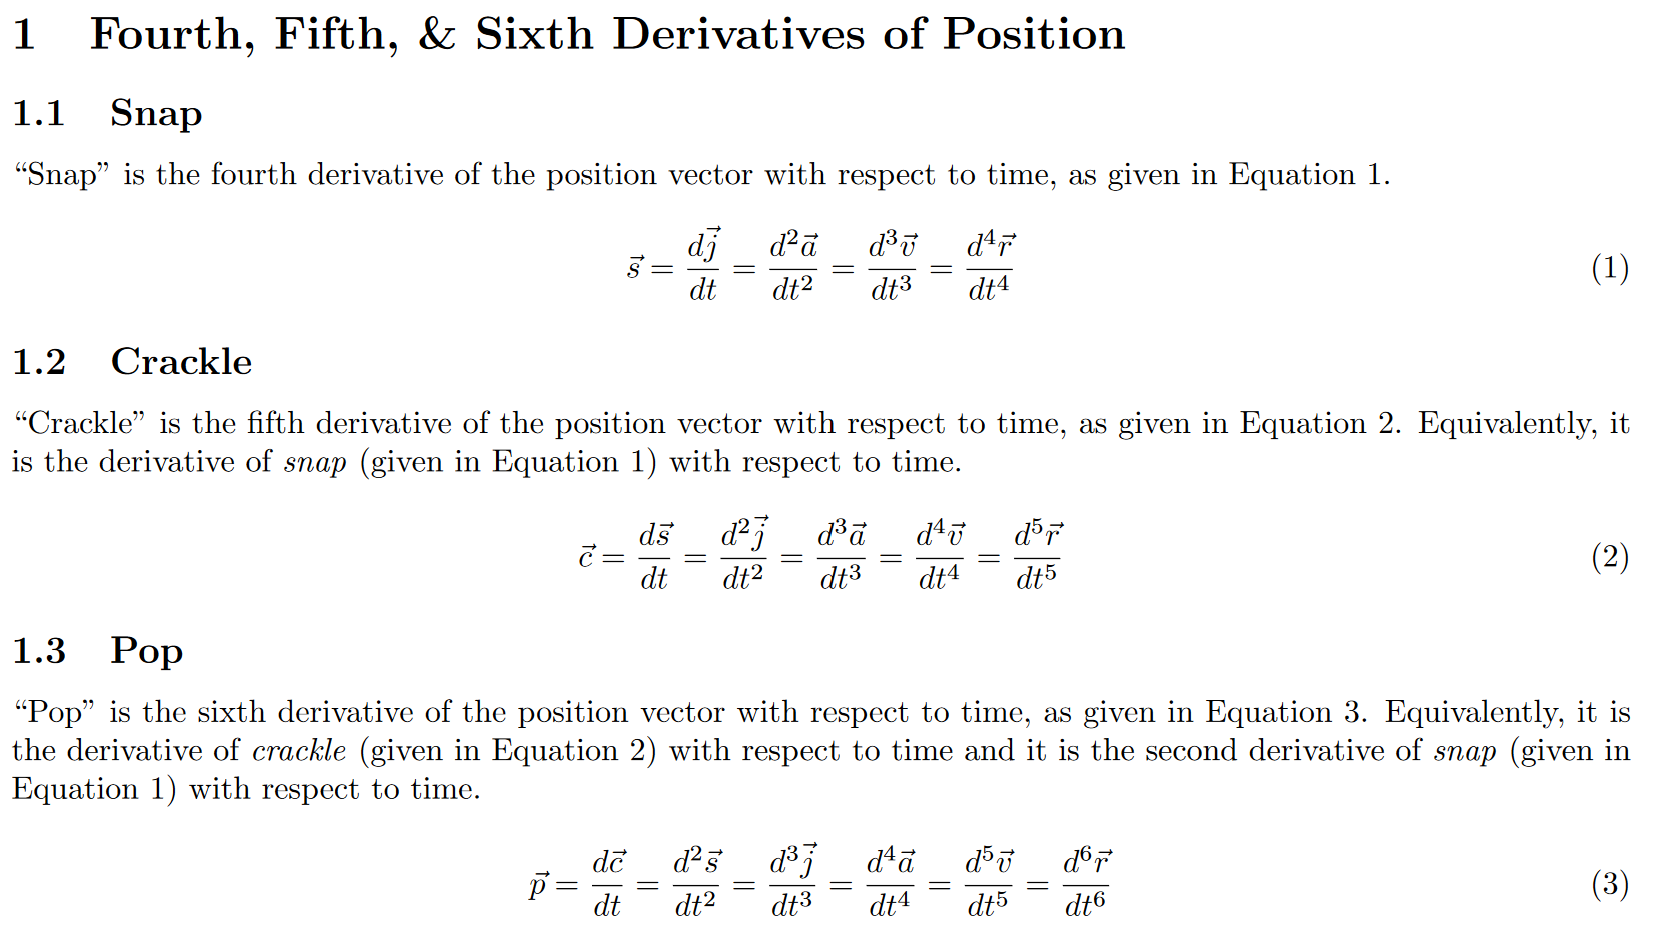
\includegraphics[width=\linewidth]{img/cereal.png}
\end{frame}


\begin{frame}[fragile]
\frametitle{Challenge: Cross-References}
\begin{alertblock}{Cross-References Source Code (1/3)}
\small
\begin{minted}{latex}
\section{Fourth, Fifth, \& Sixth Derivatives of Position}

\subsection{Snap} \label{sec:snap}

``Snap" is the fourth derivative of the position vector 
with respect to time, as given in Equation~\ref{eq:snap}.

\begin{equation} \label{eq:snap}
    \Vec{s} 
    = \frac{d\Vec{j}}{dt} = \frac{d^2 \Vec{a}}{dt^2} 
    = \frac{d^3 \Vec{v}}{dt^3} = \frac{d^4 \Vec{r}}{dt^4}
\end{equation}
\end{minted}
\end{alertblock} 
\end{frame}


\begin{frame}[fragile]
\frametitle{Challenge: Cross-References}
\begin{alertblock}{Cross-References Source Code (2/3)}
\small
\begin{minted}{latex}
\subsection{Crackle} \label{sec:crackle}

``Crackle" is the fifth derivative of the position vector 
with respect to time, as given in 
Equation~\ref{eq:crackle}. Equivalently, it is the 
derivative of \emph{snap} (given in Equation~\ref{eq:snap}) 
with respect to time.

\begin{equation} \label{eq:crackle}
    \Vec{c} 
    = \frac{d\Vec{s}}{dt} = \frac{d^2 \Vec{j}}{dt^2} 
    = \frac{d^3 \Vec{a}}{dt^3} = \frac{d^4 \Vec{v}}{dt^4} 
    = \frac{d^5 \Vec{r}}{dt^5}
\end{equation}
\end{minted}
\end{alertblock} 
\end{frame}


\begin{frame}[fragile]
\frametitle{Challenge: Cross-References}
\begin{alertblock}{Cross-References Source Code (3/3)}
\small
\begin{minted}{latex}
\subsection{Pop} \label{sec:pop}

``Pop" is the sixth derivative of the position vector with
respect to time, as given in Equation~\ref{eq:pop}. 
Equivalently, it is the derivative of \emph{crackle} 
(given in Equation~\ref{eq:crackle}) with respect to time 
and it is the second derivative of \emph{snap} (given in 
Equation~\ref{eq:snap}) with respect to time. 

\begin{equation} \label{eq:pop}
    \Vec{p} 
    = \frac{d\Vec{c}}{dt} = \frac{d^2 \Vec{s}}{dt^2} 
    = \frac{d^3 \Vec{j}}{dt^3} = \frac{d^4 \Vec{a}}{dt^4} 
    = \frac{d^5 \Vec{v}}{dt^5} = \frac{d^6 \Vec{r}}{dt^6}
\end{equation}
\end{minted}
\end{alertblock} 
\end{frame}